%%% Ne pas modifier jusqu'à la ligne 25
\documentclass[a4paper,12pt]{book}
\usepackage[utf8]{inputenc}
\usepackage[french]{babel}
%%\usepackage{CJK}
\usepackage{yhmath}
\usepackage[left=2cm,right=2cm,top=3cm,bottom=2cm, headheight=1.5cm,headsep=1.5cm]{geometry}
%%\usepackage{CJKutf8}
\usepackage{amsfonts}
\usepackage{mathrsfs}
\usepackage{amsmath,amsfonts,amssymb,dsfont}
\usepackage{graphicx}
\usepackage{subfigure}
\usepackage{enumitem}		%\enumerate-resume
\usepackage[colorlinks=true,unicode={true},hyperindex=false, linkcolor=blue, urlcolor=blue]{hyperref}
\newcommand{\myref}[1]{\ref{#1} page \pageref{#1}}

\addto\captionsfrench{\def\tablename{Tableau}}  %légendes des tableaux
\renewcommand\thesection{\Roman{section}~-~} 
\renewcommand\thesubsection{\Roman{section}.\Alph{subsection}~-~} 
\renewcommand\thesubsubsection{\Roman{section}.\Alph{subsection}.\arabic{subsubsection}~-~} 

\newcommand{\conclusion}[1]{\newline \centerline{\fbox{#1}}}

\setcounter{secnumdepth}{3}
\parindent=0pt

\usepackage{fancyhdr}
\pagestyle{fancy}

\lhead{SJTU-ParisTech} 
%%%%%%%%%%%%%%%%%%%%%%%%%%%%%%%%%%
\chead{DM4}
\rhead{Daniel 518261910024}

\begin{document}
\renewcommand{\labelitemi}{$\blacktriangleright$}
\renewcommand{\labelitemii}{$\bullet$}


\section{Activité 3-2}
\begin{figure}[h]
    \begin{center}
    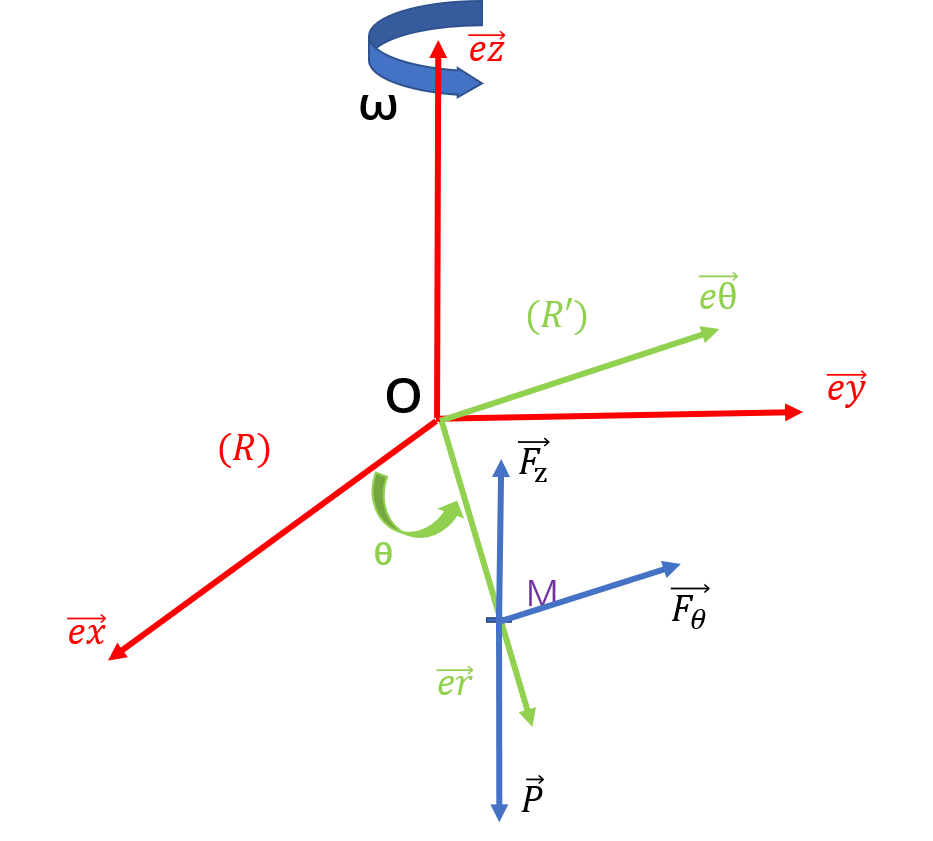
\includegraphics[scale=0.6]{meca41.png}
    \end{center}
    \caption{le système étudiée}
\end{figure}
On note $(R)$ le référentiel terrestre supposé galiléen, et $(R^{'})$ le référentiel tournant, 
$(O,\{\vec{e_x},\vec{e_y},\vec{e_z}\})$ le repère lié à $(R)$, et $(O,\{\vec{e_r},\vec{e_\theta},\vec{e_z}\})$ 
le repère lié à $(R^{'})$. 

On a $\vec{\Omega}_{(R^{'})/(R)}=\omega\vec{e_z}$
\subsection{}
système: le point matériel $M$ de masse $m$, avec $\overrightarrow{OM}=r\vec{e_r}$
Bilan des actions: 
\begin{itemize}
    \item Poids $\vec{P}=-mg\vec{e_z}$
    \item réaction exercée par les parois: $\vec{F}=F_\theta\vec{e_\theta}+F_z\vec{e_z}$
\end{itemize}
On a alors 
$$
\frac{dE_{m,(R^{'})}(M)}{dt}=P_{\vec{P}}+P_{\vec{F}}=(\vec{P}+\vec{F})\cdot d\overrightarrow{OM}
$$
On notice que $d\overrightarrow{OM}$ est toujours perpendiculaire à les forces $\vec{P}$ et $\vec{F}$, 
donc $\boxed{\frac{dE_{m,(R^{'})}(M)}{dt}=0}$, le système est donc conservatif dans $R^{'}$

On a $\vec{F}_{ext \to (M)}=-\overrightarrow{grad}E_p$, donc 
$$
\frac{\partial E_p}{\partial r}\vec{e_r}+\frac{\partial E_p}{\partial \theta}\vec{e_\theta}+\frac{\partial E_p}{\partial z}\vec{e_z}=F_\theta\vec{e_\theta}+(F_z-mg)\vec{e_z}
$$
On va démontrer plus tard que $F_z=mg$, donc on a 
$$
\frac{\partial E_p}{\partial \theta}\vec{e_\theta}=\frac{d E_p}{d \theta}\vec{e_\theta}=F_\theta\vec{e_\theta}
$$
On a finalement $\boxed{E_p=\theta F_\theta+cste}$

Le système \fbox{n'est pas conservatif} dans $(R)$ car $(R^{'})$ n'est pas en tranlation avec $(R)$

\subsection{}
On a $\overrightarrow{OM}=r\vec{e_r}$, donc 
$$
\vec{v}_{(R^{'})}(M)=\left(\frac{d\overrightarrow{OM}}{dt}\right)_{(R^{'})}=\dot{r}\vec{e_r}, \quad 
\vec{a}_{(R^{'})}(M)=\left(\frac{d\vec{v}_{(R^{'})}(M)}{dt}\right)_{(R^{'})}=\ddot{r}\vec{e_r} 
$$
Et on a 
$$
\vec{a}_e(M)=-\omega^2r\vec{e_r}, \quad \vec{a}_c(M)=2\omega\vec{e_z} \wedge \dot{r}\vec{e_r}=2\omega \dot{r}\vec{e_\theta}
$$
On applique PFD sur M dans $(R)$: 
\begin{align*}
m\ddot{r}\vec{e_r}&=\vec{P}+\vec{F}+\vec{F}_{ie \to M}+\vec{F}_{ic \to M}\\
&=m\omega^2r\vec{e_r}+(F_\theta-m^2\omega\dot{r})\vec{e_\theta}+(F_z-mg)\vec{e_z}
\end{align*}
En faisant les projections sur $\vec{e_r}$, $\vec{e_\theta}$ et $\vec{e_z}$, on obtient 
$$
m\ddot{r}=m\omega^2r, \quad F_\theta=m^2\omega\dot{r}, \quad F_z=mg
$$
Donc on a $\boxed{\ddot{r}-\omega^2r=0}$. 

On a donc $r=C_1 e^{\omega t}+C_2 e^{-\omega t}$, avec les conditions initiaux $r(t=0)=\frac{L}{2}$, $\dot{r}(t=0)=0$. 
Ainsi, on a $C_1=C_2=\frac{L}{4}$. 

Finalement, on a $\boxed{r=\frac{L}{4}(e^{\omega t}+e^{-\omega t})}$

\subsection{}
Il faut que $r(t=T)=\frac{L}{4}(e^{\omega T}+e^{-\omega T})=L$, et nécessairement $T\geq 0$. 

On obtient donc $\boxed{T=\frac{\ln(2+\sqrt{3})}{\omega}}$
\subsection{}
On a déjà $F_\theta=m^2\omega\dot{r}, F_z=mg$. Donc la réaction exercée par les parois 
est $\boxed{\vec{F}=m^2\omega\dot{r}\vec{e_\theta}+mg\vec{e_z}}$

\section{Exercice 4-5}
Le repère: $(O,\{\vec{e_r},\vec{e_\theta},\vec{e_z}\})$
\begin{figure}[h]
    \begin{center}
    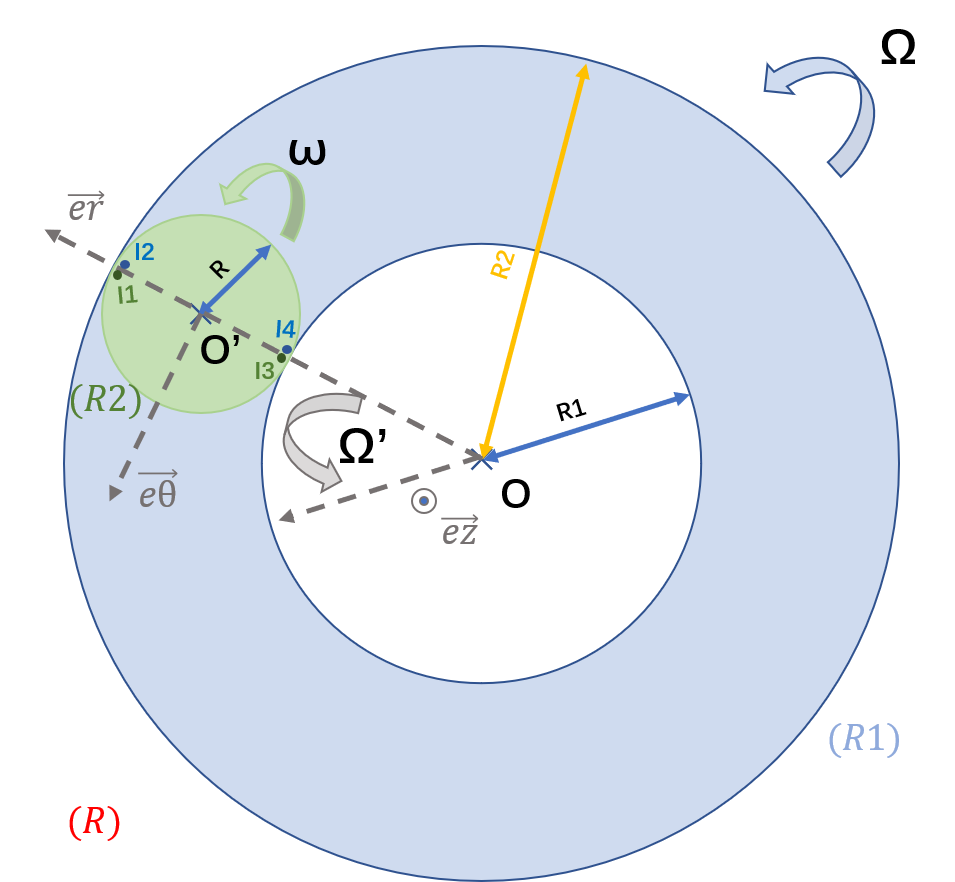
\includegraphics[scale=0.6]{meca42.png}
    \end{center}
    \caption{le système étudiée}
\end{figure}
\subsection{}
Les systèmes:
\begin{itemize}
    \item $(R)$: le système terrestre supposé galiléen
    \item $(R_1)$: le système tournant lié au cylindre extérieur
    \item $(R_2)$: le système tournant lié à la bille
    %\item $(R_3)$: le système tournant lié au cylindre intérieur
\end{itemize}
Les vecteurs rotations:
\begin{itemize}
    \item $\vec{\Omega}_{(R_1)/(R)}=\Omega \vec{e_z}$, avec $\Omega$ la vitesse angulaire du cylindre extérieur
    \item $\vec{\Omega}_{(R_2)/(R)}=\omega \vec{e_z}$, avec $\omega$ la vitesse angulaire de la bille
    \item $\Omega^{'}$: la vitesse angulaire du $O^{'}$ par rapport à $O$
\end{itemize}
Les points:
\begin{itemize}
    \item $I_1$: Le point lié à la bille, qui coïncide avec $I_2$ à l'instant étudié 
    \item $I_2$: Le point lié au cylindre extérieur, qui coïncide avec $I_1$ à l'instant étudié 
    \item $I_3$: Le point lié à la bille, qui coïncide avec $I_4$ à l'instant étudié 
    \item $I_4$: Le point lié au cylindre intérieur, qui coïncide avec $I_3$ à l'instant étudié 
\end{itemize}
Pour un contact sans glissement entre la bille et le cylindre intérieur, il faut que $\vec{v}_{(R)}(I_3)=\vec{v}_{(R)}(I_4)$. 
on a 
\begin{align*}
\vec{v}_{(R)}(I_3)&=\vec{v}_{(R_2)}(I_3)+\vec{v}_{(R)}(O^{'})+\vec{\Omega}_{(R_2)/(R)}\wedge \overrightarrow{O^{'}I_3}\\
&=\vec{0}+\Omega^{'}(R+R_1)\vec{e_\theta}+\omega \vec{e_z}\wedge (-R)\vec{e_r}\\
&=[\Omega^{'}(R+R_1)-R\omega]\vec{e_\theta}
\end{align*}
Comme $I_4$ est immobile, on a $\Omega^{'}(R+R_1)-R\omega=0$

Pour un contact sans glissement entre la bille et le cylindre extérieur, il faut que $\vec{v}_{(R)}(I_1)=\vec{v}_{(R)}(I_2)$. 
on a
\begin{align*}
\vec{v}_{(R)}(I_2)&=\vec{v}_{(R_2)}(I_2)+\vec{\Omega}_{(R_1)/(R)}\wedge \overrightarrow{OI_2}\\
&=(\Omega R_2)\vec{e_\theta}
\end{align*}
Et
\begin{align*}
    \vec{v}_{(R)}(I_1)&=\vec{v}_{(R_2)}(I_1)+\vec{v}_{(R)}(O^{'})+\vec{\Omega}_{(R_2)/(R)}\wedge \overrightarrow{O^{'}I_1}\\
    &=\vec{0}+\Omega^{'}(R+R_1)\vec{e_\theta}+\omega \vec{e_z}\wedge (R)\vec{e_r}\\
    &=[\Omega^{'}(R+R_1)+R\omega]\vec{e_\theta}
\end{align*}
Donc on a $\Omega^{'}(R+R_1)+R\omega=\Omega R_2$

Finalemant, on obtient 
$$\boxed{\Omega^{'}=\frac{\Omega R_2}{2(R+R_1)}, \quad \omega=\frac{\Omega R_2}{2R}}$$

\subsection{}
On a $E_{c,tot}=E_{c,(R_1)}+E_{c,(R_2)}$, avec
$$
E_{c,(R_1)}=\frac{1}{2}I_{\Delta}(R_1)\Omega^2=\frac{1}{2}R_2^2m_2\Omega^2
$$
et on a  
\begin{align*}
I_{\Delta}(R_2)&=\int_{(\Sigma)}d^2_{p,\Delta}dm_P\\
&=\int_{r \in [0,R], \theta \in [0,2\pi[}\rho [(r+R_1)^2+r^2+2r(r+R_1)\cos\theta]r\,drd\theta\\
&=\frac{3m}{2R}\left(\frac{R^2}{2}+\frac{2}{3}R_1R+\frac{1}{2}R_1^2\right)
\end{align*}
Finalement, 
$$
\boxed{E_{c,tot}=\frac{1}{2}R_2^2m_2\Omega^2+N\left(\frac{\Omega R_2}{2(R+R_1)}\right)^2\frac{3m}{4R}\left(\frac{R^2}{2}+\frac{2}{3}R_1R+\frac{1}{2}R_1^2\right)}
$$


\end{document}